
TVB is logically and technically divided at deploy time into a scientific library and a framework package, 
where the scientific library includes datatypes, basic analyses and the simulator as its central piece,
while the framework handles execution infrastructure, the web-based user interface and data storage. 
 TVB Scientific Library can function independently, as a Python module, but TVB Framework needs 
the scientific library to wrap around it at runtime.

TVB source code is available for download on Github at \url{https://github.com/the-virtual-brain/}. 
Previous Git and Python knowledge is required for contributing.
Although you could independently install Python and the rest of TVB dependencies on your machine, 
and then use the Github code as a simple local clone, we recommend you to download \emph{TVB\_ Distribution}
from \url{http://www.thevirtualbrain.org/register/}, fork our repositories on Github and further use
\emph{contributor\_setup} script, from inside \emph{TVB\_ Distribution} folder, to link the two. 
In this recommended use-case, you will have all TVB dependencies already prepared and at your disposal, 
as part of \emph{TVB\_Distribution}.

 \begin{figure*}
        \centering
        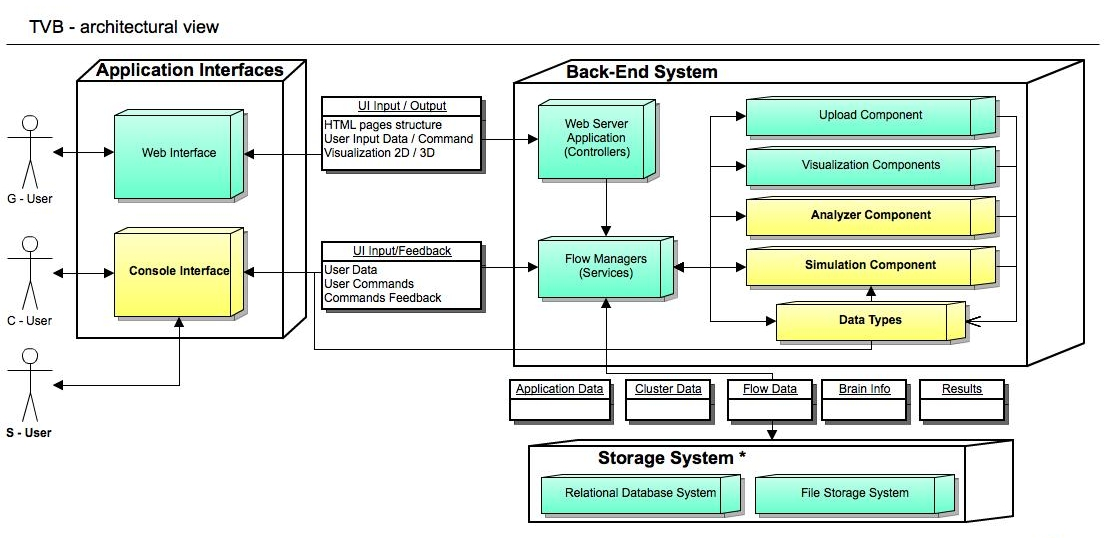
\includegraphics[width=0.90\textwidth]{images/architecture.jpg}
        \caption{TVB architecture: 
        Yellow blocks are part of the Scientific Library of TVB, while the green blocks are part of TVB Framework.
        TVB provides two independent interfaces, depending on the interaction type wanted by the end-user (web or console).
        TVB Storage layer is compulsory for the web interface, but it can be switched on/off for the console interface.
         }
        \label{fig:architecture}
 \end{figure*}

	\subsection{Basic Concepts}

TVB has been developed with generality and modularity in mind. The central idea is data-oriented in a sense that
data is fed and stored into the system and can be transformed into another type
of data (including visualization) through operations provided by an external
library (including TVB scientific library, but not restricted to it) that have
been \emph{adapted} to the framework. As a consequence, central concepts in TVB
are \emph{datatypes} i.e. types of data that can be handled in the framework and
\emph{adapters} i.e. classes that allow to interface/adapt external libraries
to  the datatypes handled by within the framework.

	\subsubsection{TVB Traits}

System is inspired by the traiting module developed by Enthought \cite{Enthought_2001}.
Out traiting system offers a way to annotate fields and classes from inside TVB, with specific trait-attributes,
which will be further used in different layers of the application.
Trait-attributes are synonym with meta-data for TVB classes and their fields.

Because an explicit goal of TVB was to provide a user interface to each of the
entities and algorithms contained within, it is necessary at some point to
provide metadata on how to built that interface. A \texttt{traits} system was developed, similar to that of
IPython or EPD, was developed, allowing for fields on a TVB class to
be written out with full metadata on it. An extensive set of  building 
blocks are already implements from numeric types and arrays to lists, tuples, 
string, and dictionaries.

 When methods of such a class with annotated fields are invoked,
they may use the traited-attributes directly, accessing either a default value
or one given during the instantiation of the object. Additionally, this allows
the web-based user interface to introspect a class for all of its fields and their
descriptions, to provide help and choose the proper display form. The explicit typing also allows
such classes to be nearly automatically mapped to storage tables,
thus providing smooth persistence, when the storage layer is enabled.  
Lastly, because such metadata is used to build the docstring of a class,
the IPython user also may obtain extensive descriptions of class, fields, methods and
arguments in the usual way. 

So, we have trait-attributes for describing how a certain class with its fields 
will be stored in the database and the file-storage system,
for describing display manners in the web-interface, for documenting fields or classes, 
and even meta-data on what valid values are allowed on a certain field. 
The complete list of currently supported traited-attributes is described in Table \ref{tab:traits}.

\begin{center}
	\begin{table*}[ht]
  	\label{tab:traits}
  	\caption{TVB currently available Traited Attributes}

	\begin{tabularx}{\textwidth}{lll}
      		\toprule
      		Traited Attribute    & Description  \\ 
      		\midrule
		default 	& Default value for current field. Will be set on any new instance if not specified otherwise in the constructor.  \\
		console\_default & Define how a default value can be computed for current field, when console interface is enabled. \\
		range	& Specify the set of accepted values for current field. Mark that this field is usable for parameter space exploration. \\

		label		& Short text to be displayed in UI, in front of current field. \\
		doc		& Longer description for current field. To be displayed in UI as help-text. \\
		required	& Mark current field as required for when building a new instance of the parent class. \\
		locked	& When present and \emph{True}, current field will be displayed as read-only in the web interface. \\

		options	& Attribute present for fields of type \emph{Enumerate}, specifying the accepted options as a list of strings. \\
		filters\_ui	& Filters towards other fields, to be applied in UI. \\
		select\_multiple & When \emph{True}, current field will be displayed as a select  with multiple options in UI (default is single-select) \\
		order	& Optional number identifying the index at which current field will be displayed in UI. \\
				& When negative, the field is not displayed at all. Ascending order for indices is considered when displaying. \\

		use\_storage	& When \emph{False}, current field is not stored in database or file storage. \\
		file\_storage	& Valid values for this attribute are: \emph{None} , \emph{HDF5}, or  \emph{expandable\_HDF5}, \\
					& When \emph{None}, current field is not stored in the file-storage at all. When \emph{HDF5}, we use regular H5 file storage. \\
					& When \emph{expandable\_HDF5} value is set, a H5 stored in chuncks is used. \\
		\bottomrule
    	\end{tabularx}
	\end{table*}
\end{center}


	\subsubsection{DataTypes}

In TVB, DataTypes represent the common language, to be used between different other application parts: 
like uploaders, analyzers, simulator and visualizers.
Some of the algorithms are producing these DataTypes, while others are reading them as input. 
In order to decouple the definition and several usages of such entities, DataTypes are declared outside the algorithms 
and shared between them. For example an instance of datatype TimeSeriesRegion is created by the Simulator, 
and it can be accepted as input for several visualizers or analyzed by PCA and Cross Coherence algorithms.

In a more technical definition, TVB DataTypes are annotated structures (Python classes), which
contain one or more fields and associated descriptive information, as
well as methods for operating on the data they contain. The definition of a
DataType is achieved using TVB's traiting system, mentioned in previous section.

In scientific Python code, it is conventional to provide arguments
of an algorithm as a ``bare'' array or collection there of, and sanity
checks of arguments proceed on the basis of array geometry, for example.
In TVB, we consider a \textit{DataType} to be a full, formal description of 
an entity involved in an algorithm that would be part of TVB. 
For example, the \texttt{Connectivity} DataType, which may elsewhere
be represented by a simple $N$ by $N$ NumPy array, is written as a class
in which one of the attributes, \texttt{weights}, is a explicitly typed 
\texttt{FloatArray}, and the declaration of this type is complemented by
explicit label, default values, and documentation strings. 

\begin{lstlisting}
class ConnectivityData(MappedType):

  region_labels = arrays.StringArray( 
	label="Region labels", 
        doc="""Labels for the regions ...""")

  weights = arrays.FloatArray( 
	label="Connection strengths",
        doc="""... strength of connections ...""")

  tract_lengths = arrays.FloatArray( 
	label="Tract lengths",
        doc="""... length of myelinated fibre tracts.""")

   speed = arrays.FloatArray( 
	label="Conduction speed", 
	default=numpy.array([3.0]), 
	file_storage=core.FILE_STORAGE_NONE,
         doc="""... matrix of conduction speeds ...""")

  centres = arrays.PositionArray( 
	label="Region centres",
        doc="""... locations for the region centers""")
\end{lstlisting}

	\subsubsection{Profile}

TVB uses the notion of \emph{profile} to identify in what context the application is currently running,
and thus what components are expected to be plugged and how.

For example, when TVB scientific library is used alone, a specific profile (\emph{library profile}) class 
gets linked as current profile, which, in this case, disables data storage and the web interface. Other profiles available
in TVB are: \emph{command profile}, \emph{deployment profile} (with web interface), and \emph{test profiles}.

	\subsection{TVB Scientific Library}

	\subsubsection{General description}

	\subsubsection{TVB Specific Datatypes}

\note[lp]{Table 2 ``TVB datatypes'' of FIN article might be interesting here?}

	\subsection{TVB Framework}

	\subsubsection{General description}

TVB framework provides a storage back-end, workflow management and a number of features to
support collaborative work. The framework supports two user interfaces: web-based graphical interface or the
console interface for advanced user and developers.

Due to the generality of the framework, it relies on the Python \emph{abstract classes} mechanism.
\note[lp]{From Python glossary:}
Abstract base classes complement duck-typing by providing a way to define
interfaces when other techniques like hasattr() would be clumsy or subtly wrong.

\subsubsection{Data Storage}

We are storing data both in the file system and in a relational database.
The file system is for storing big chunks of data, and the relational database is mainly for quick indexing, 
and storing entities which are used at display time in the web interface.

The relational database management is done from the code by using \emph{SQLAlchemy} \texttt{http://www.sqlalchemy.org/}, 
which offers a transparent manner to connect underneath to either: SQLite or PostgreSQL, as the user chooses at install time.
When choosing PostgreSQL, the end-user needs to separately install and configure the database, and provide in TVB
interface only the URL for connection.

\note[ld]{Write more details here. E.g. about GIDs}


\subsubsection{Adapters}

While DataTypes provide a way of description what data do algorithms work with, 
sufficing for the typical user looking to write scripts against the
available libraries, TVB framework requires algorithms to adhere to 
a generic interface, which is elsewhere referred to as the Adapter pattern.
Typically, this implies that a class is written that is able to describe
the collection to datatypes required and a single method to invoke the
algorithm.

Adapters are derived from the abstract class named \texttt{ABCAdapter} which
defines the common interface for the adapters with compulsory methods to be implemented like:

\begin{lstlisting}
class ABCAdapter(object):

  @abstractmethod
  def get_input_tree(self):

  @abstractmethod
  def get_output(self):

  @abstractmethod
  def get_required_memory_size(self, **kwargs):

  @abstractmethod
  def get_required_disk_size(self, **kwargs):

  def get_execution_time_approximation(self, **kwargs):

  def configure(self, **kwargs):

  @abstractmethod
  def launch(self):
\end{lstlisting}

Several categories of adapters have been defined in TVB: 

\begin{itemize}
	\item \textit{creators} which are internal algorithms for producing DataType instances. 
		Each creator has one or multiple pages in the web interface, in which the user
		 configures input parameters and chooses from the available options for computing a particular DataType.

	\item \textit{uploaders}: allow the upload into TVB framework of external data, 
    		such as \emph{gifti} files of plain \emph{csv} files.

	\item \textit{simulator} is an adapter wrapping over TVB simulator library, and adjusting it to fit
		the workflow mechanisms inside TVB framework .

	\item \textit{analyzers} which offer the interface between libraries containing algorithms 
		for the analysis of the data (wavelets, FastICA, BCT, etc.) and the TVB framework and datatypes.

	\item \textit{visualizers} are derived from the \emph{ABCDisplayer} abstract class, and are preparing  
		a DataType instance for display. Each Visualizer (Python adapter class) requires a complementary set
		of JS and HTML files for managing the actual display of data.

	\item \textit{portlets} are wrapper classes for a chain of analyzers and a visualizer at the end of the chain.

	\item \textit{exporters} are utility classes for preparing data in TVB (DataType or group of DataTypes)
		before export (web download).
\end{itemize}

Note that the adapters and datatypes are intended to provide full 
power and flexibility of the framework; when the simulator is invoked from
the web-based UI, it is done so through an \texttt{SimulatorAdapter} which,
despite being relatively complex, is build with \emph{traits} all the way down.

It is reasonable to ask what such a scheme offers over the more 
conventional approach of Python, where presumably it would have been
sufficient that each adapter consist of a class with an \texttt{\_\_init\_\_}
and \texttt{\_\_call\_\_} method, in the case of a function type. 
We note that because in the case of TVB, the context in which an object
is used is more varied, e.g. not simply initialized but loaded through 
SqlAlchemy's ORM, and that the adapter is required to perform more tasks
than just initialization and invocation, e.g. provide expected shape of 
result, estimate occupied memory and do not start if insufficient resources are found on current machine,
 it was advantageous to create a distinct set of interfaces built on top of
the abstract base class framework provided by Python's standard library.

\paragraph{Adapting sklearn's FastICA}

\note[mw]{Show the adapter for FastICA}

\paragraph{Interfacing with MATLAB}

One of the well-known libraries for characterizing anatomical 
and functional connectivity is the \emph{Brain Connectivity Toolbox} 
\cite{Rubinov_2010}. 
Because it is written in MATLAB, with maintainers who prefer MATLAB, we 
chose not to port routines of the library to Python but instead build
a MATLAB adapter which runs arbitrary MATLAB code. 

This generic Matlab adapter works by generating at runtime a script with MATLAB code, 
wrapping the script call in Python with a try-except clause,  
loading and saving the workspace before and after the call,
generating a workspace \texttt{.mat} file, invoking the MATLAB or Octave
executable, and loading the resulting workspace file. 

Despite invocation of MATLAB being a relatively slow operation, this works fine in a single
user situation, and where Octave is available, it is quite fast. In the 
case that many operations are necessary, they can be batched into the 
same run.

\subsection{Documentation}

We provide an API doc, built from the docs strings using Sphinx.
Users, Contributors and Developers manuals are also provided with TVB
distributions in pdf format. The source files (in .rst) are available
through the github repository \url{https://github.com/the-virtual-brain/docs}.  
In addition, IPython \cite{PerezGranger_2007} notebooks
for interactive tutorials are provided. These are based on the
demonstration scripts provided with the scientific library, and
include a more detailed description of what the scientific goal is (if
applicable), the components and stages of a simulation as well as a
brief description in the case of reproducing previous work. Users
interacting with \TVB GUI may also benefit from these tutorials
(\url{links: https://github.com/the-virtual-
brain/scientific_library/wiki/Tutorials}) when displayed as snippets
with Ipython nbviewer. 

The user interface provides an online help overlay, that pulls
information from the Users manual.


